\documentclass[border=4pt]{standalone}
\usepackage{tikz}
\usetikzlibrary{arrows,positioning}
\begin{document}
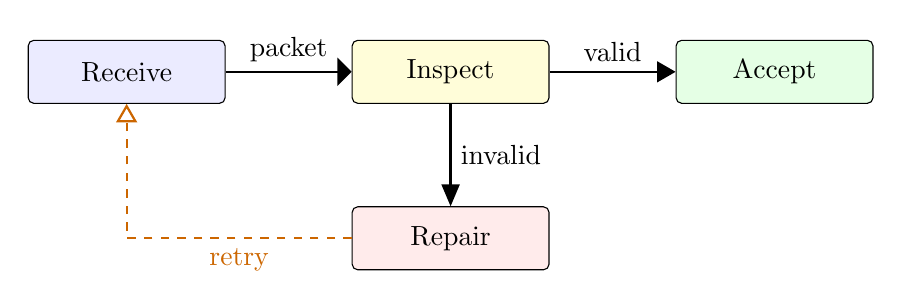
\begin{tikzpicture}[
  node distance=13mm and 16mm,
  task/.style={draw,rounded corners=2pt,minimum width=25mm,minimum height=8mm,align=center},
  route/.style={line width=.8pt}
]
  \node[task,fill=blue!8] (receive) {Receive};
  \node[task,fill=yellow!15,right=of receive] (inspect) {Inspect};
  \node[task,fill=green!10,right=of inspect] (accept) {Accept};
  \node[task,fill=red!8,below=of inspect] (repair) {Repair};

  \draw[route,-{triangle 90}] (receive) -- node[above]{packet} (inspect);
  \draw[route,-{triangle 60}] (inspect) -- node[above]{valid} (accept);
  \draw[route,-{triangle 45}] (inspect) -- node[right]{invalid} (repair);
  \draw[route,dashed,orange!80!black,-{open triangle 60}]
    (repair.west) -| node[pos=.25,below]{retry} (receive.south);
\end{tikzpicture}
\end{document}
